\usetikzlibrary{%
	matrix,%
	calc,%
	arrows%
}
\chapter{BẤT BIẾN ĐỒNG LUÂN}

\indent Chúng ta sẽ chứng minh đồng điều kỳ dị là các không gian tương đương đồng luân có các nhóm đồng điều đẳng cấu. Điều này sẽ được thực hiện bởi chỉ ra rằng một ánh xạ \(f: X \rightarrow Y\) tạo ra một phép đồng cấu cảm sinh  \(f_{\textasteriskcentered} : H_n(X)→H_n(Y)\) cho mỗi \(n\), và \(f_{\textasteriskcentered}\) là một đẳng cấu nếu \(f\) là một phép đồng cấu tương đương. \\
\indent Đối với ánh xạ \(f: X \rightarrow Y\) , một phép đồng cấu cảm sinh \(f_{\sharp} : C_n(X) \rightarrow C_n(Y)\) được xác định bằng  cách  kết  hợp  từng  \(n\) - đơn  hình  kỳ dị \(\sigma : \Delta_{n} \rightarrow X\) với  \(f\)  để  nhận  được \(n\) - đơn  hình  kỳ  dị  \(f_{\sharp}(\sigma) = f\sigma : \Delta^{n} \rightarrow Y\) , sau đó mở rộng \(f_\sharp\) tuyến tính qua \(f_{\sharp}(\sum_{i}n_{i}\sigma_i) = \sum_{i}n_{i}f_{\sharp}(\sigma_i) = \sum_{i}n_{i}f\sigma_i\) . Ánh xạ \(f_{\sharp} : C_n(X) \rightarrow C_n(Y)\) thỏa mãn \( f_{\sharp}\partial = \partial f_{\sharp}\), khi đó:
\begin{equation*}\label{eq:pareto mle2}
\begin{aligned}
f_{\sharp}\partial(\sigma) & = f_{\sharp}(\sum_{i}(-1)^{i}\sigma|[v_0,\cdots,\hat{v}_{i},\cdots,v_n]) \\
& = \sum_{i}(-1)^{i}f\sigma|[v_0,\cdots,\hat{v}_{i},\cdots,v_n] \\
& = \partial f_{\sharp}(\sigma)
\end{aligned}
\end{equation*}
\newpage
Vì vậy, ta có biểu đồ: \\
\begin{tikzpicture}[>=triangle 60]
	\matrix[matrix of math nodes,column sep={60pt,between origins},row sep={60pt,between origins},nodes={asymmetrical rectangle}] (s)
	{
		|[name=A0]| \cdots &|[name=A1]| C_{n+1} &|[name=A2]| C_n &|[name=A3]| C_{n-1} &|[name=A4]| \cdots \\
		%
		|[name=B0]| \cdots &|[name=B1]| C_{n+1} &|[name=B2]| C_n &|[name=B3]| C_{n-1}  &|[name=B4]| \cdots\\
	};
	\draw[->] (A0) edge (A1)
	(A1) edge node[auto] {$\partial$} (A2)
	(A2) edge node[auto] {$\partial$} (A3)
	(A3) edge (A4)
	(A1) edge node[auto] {\(f_{\sharp}\)} (B1)
	(A2) edge node[auto] {\(f_{\sharp}\)} (B2)
	(A3) edge node[auto] {\(f_{\sharp}\)} (B3)
	(B0) edge (B1)
	(B1) edge node[auto] {$\partial$} (B2)
	(B2) edge node[auto] {$\partial$} (B3)
	(B3) edge (B4)
	;
\end{tikzpicture} \\
sao cho, \( f_{\sharp}\partial = \partial f_{\sharp}\). Một biểu đồ của bản đồ với thuộc tính mà sự hợp thành của hai ánh xạ bất kỳ bắt đầu tại một điểm trong biểu đồ và kết thúc ở một biểu đồ khác bằng nhau được gọi là \textbf{biểu đồ giao hoán}. Trong trường hợp hiện tại tính giao hoán của giản đồ tương đương với quan hệ giao hoán \( f_{\sharp}\partial = \partial f_{\sharp}\) , nhưng biểu đồ giao hoán có thể chứa tam giác giao hoán, ngũ giác, v.v., cũng như bình phương giao hoán. \\
\indent Thực tế là các ánh xạ \(f_{\sharp} : C_n(X) \rightarrow C_n(Y)\) thỏa mãn \( f_{\sharp}\partial = \partial f_{\sharp}\) cũng được thể hiện bằng cách nói rằng \(f_{\sharp}\) xác định ánh xạ dây chuyền từ phức hợp dây chuyền kỳ dị của \(X\) của \(Y\) . Hệ thức \( f_{\sharp}\partial = \partial f_{\sharp}\) ngụ ý rằng \(f_{\sharp}\) đưa chu trình đến chu trình khi \(\partial_{\alpha} = 0\) ngụ ý \(\partial(f_{\sharp}\alpha) = f_{\sharp}(\partial\alpha) = 0\) . Ngoài ra, \(f_{\sharp}\) đưa biên đến biên khi \(f_{\sharp} (\partial\beta) = \partial(f_{\sharp}\beta)\). Do đó \(f_{\sharp}\) tạo ra một đồng cấu \(f_{\textasteriskcentered} : H_n(X) \rightarrow H_n(Y)\). Một mệnh đề đại số của điều ta vừa chứng minh là:

\section{Mệnh đề}
\indent Một ánh xạ dây chuyền giữa các phức hợp dây chuyền đồng cấu cảm sinh giữa các nhóm đồng điều của hai phức hợp.

\section{Tính chất}
\indent Hai tính chất cơ bản của  đồng cấu cảm sinh rất quan trọng mặc dù khá tầm thường là:
(i)  \((fg)_{\textasteriskcentered}\) = \(f_{\textasteriskcentered}g_{\textasteriskcentered}\) đối với ánh xạ \(X \xlongrightarrow[]{g} Y \xlongrightarrow[]{f} Z \). Điều này là  từ tính kết hợp của các dãy phức \(\Delta^{n} \xlongrightarrow[]{\sigma} X \xlongrightarrow[]{g} Y \xlongrightarrow[]{f} Z\) . \\
(ii)  \(\mathds{L}\) = \(\mathds{L}\) trong đó \(\mathds{L}\) ký hiệu ánh xạ đồng nhất của một không gian hoặc một nhóm. \\
Ít tầm thường hơn, chúng ta có:

\section{Định lý}
\indent Nếu   hai   ánh   xạ   \(f , g : X \rightarrow Y\)   đồng   luân  thì   chúng   có   cùng   đồng   cấu   cảm   sinh \( f_{\textasteriskcentered} = g_{\textasteriskcentered} : H_n(X) \rightarrow H_n(Y)\).
Theo \textbf{tính chất 3.2} , điều này ngay lập tức ngụ ý

\section{Hệ quả}
\indent Các ánh xạ \(f_{\textasteriskcentered} : Hn_(X) \rightarrow H_n(Y)\) được tạo ra bởi một sự tương đương đồng luân \(f : X \rightarrow Y\) là các đẳng cấu với mọi n. \\
\indent Quay trở lại \textbf{chứng minh định lý 3.3} \\
\begin{wrapfigure}[13]{r}[34pt]{5.5cm} 
\centering
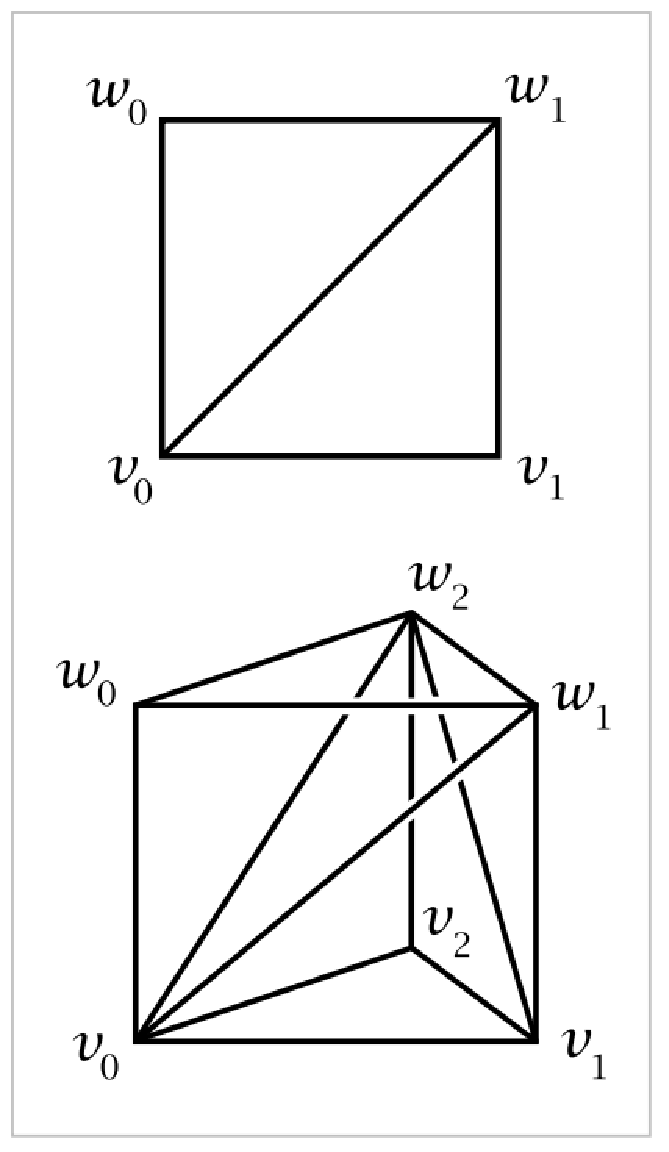
\includegraphics[scale=0.3]{figures/chap3_1}
\caption[chứng minh định lý 3.3]{chứng minh định lý 3.3
\label{fig:chap3_1}}
\end{wrapfigure}
\indent Ta chia nhỏ \(\Delta^{n} \times I\) thành các đơn hình. \textbf{Hình 3.4.1} cho thấy trường hợp \(n\) = 1, 2. Trong \(\Delta^{n} \times I\), đặt \(\Delta^{n} \times \{0\} = [v_0, \cdots , v_n]\) và \(\Delta^{n} \times \{1\} = [w_0, \cdots , w_n]\), trong đó \(v_i\) và \(w_i\) có ảnh giống nhau dưới phép chiếu \(\Delta^{n} \times I \rightarrow \Delta^n\). Ta đi từ \([v_0, \cdots , v_n]\) đến \([w_0, \cdots , w_n]\) bằng cách nội suy một dãy \(n\) - đơn hình, mỗi cái sau thu được từ cái trước bằng cách di chuyển một đỉnh \(v_i\) lên \(w_i\), bắt đầu bằng \(v_n\) và quay ngược về \(v_0\). Do đó, bước đầu tiên là di chuyển \([v_0, \cdots , v_n]\) lên \([v_0, \cdots , v_{n-1}, w_n]\), sau đó bước thứ hai  là  di  chuyển  giá  trị  này  lên  \([v_0, \cdots , v_{n-2}, w_{n-1}, w_n]\)  và  tiếp  tục  làm tương tự. Khi \([v_0, \cdots , v_i,w_{i+1}, \cdots, w_n]\) di chuyển đến \([v_0, \cdots , v_{i-1},wi, \cdots, w_n]\). Miền giữa hai \(n\)- đơn hình này chính xác là (\(n\)+1) đơn hình \([v_0, \cdots , v_i,wi, \cdots, w_n]\) có \([v_0, \cdots , v_i,w{i+1}, \cdots, w_n]\) làm mặt dưới  và \([v_0, \cdots , v_{i-1},wi, \cdots, w_n]\) làm  mặt  trên. Nhìn  chung, \(\Delta^n \times I\)  là  hợp  của  (\(n\)+1)- đơn hình \([v_0, \cdots , v_i,wi, \cdots, w_n]\)], giao nhau trong \(n\) mặt đơn hình. \\
\indent Cho một đồng luân \(F : X \times I \rightarrow Y\) từ \(f\) đến \(g\) và một đơn hình đồng điểu \(\sigma : \Delta^{n} \rightarrow X\) ,chúng ta có sự hợp thành dạng \(F ◦ (\sigma \times \mathds{L} ) : \Delta_{n} \times I \rightarrow X \times I \rightarrow Y\) . Sử dụng điều này, chúng ta có thể xác định \emph{toán tử lăng trụ} \(P : C_n(X)→C_{n+1}(Y)\) theo công thức sau: \\
\[P(\sigma) = \sum_{i} (-1)^{i}F◦(\sigma \times \mathds{L}) | [v_0, \cdots,v_i,w_i,\cdots,w_n]\]
\indent Ta sẽ chỉ ra rằng các toán tử lăng trụ này thỏa mãn hệ thức cơ bản \\
\[\partial P = g_{\sharp} - f_{\sharp} - P\partial\]
\indent Về mặt hình học, phía bên trái của phương trình này đại diện cho biên của lăng trụ và ba số hạng ở phía bên phải đại diện cho đỉnh \( \Delta^{n} \times \{1\}\), đáy \(\Delta_{n} \times \{0\}\) và các cạnh \(\partial \Delta^{n} \times I\) của lăng trụ. Để chứng minh quan hệ ta tính: \\
\begin{equation*}\label{eq:pareto mle2}
	\begin{aligned}
		\partial P(\sigma) & = \sum_{j \leq i}(-1)^{i}(-1)^{j}F\circ(\sigma \times \mathds{L}) | [v_0, \cdots, \hat{v}_j,\cdots,v_i,w_i,\cdots,w_n] \\
		& + \sum_{j \geq i}(-1)^{i}(-1)^{j+1}F\circ(\sigma \times \mathds{L}) | [v_0, \cdots, v_i,w_i,\cdots,\hat{v}_j,\cdots,w_n] \\
	\end{aligned}
\end{equation*} \\
\indent Các số hạng với i = j trong hai tổng triệt tiêu ngoại trừ \(F\circ(\sigma \times \mathds{L}) | [\hat{v}_0,w_0,\cdots,w_n]\) với \(g \circ \sigma = g_{\sharp}(\sigma)\) và \(-F\circ(\sigma \times \mathds{L}) | [v_0,\cdots,v_n,\hat{w}_n]\) với  \(-f\circ\sigma=-f_{\sharp}\). Các số hạng với \(i \neq j\) chính xác là -\(P\partial(\sigma)\), khi đó \\
\begin{equation*}\label{eq:pareto mle2}
	\begin{aligned}
		\partial P(\sigma) & = \sum_{i \leq j}(-1)^{i}(-1)^{j}F\circ(\sigma \times \mathds{L}) | [v_0, \cdots, v_i,w_i,\cdots,\hat{w}_j,\cdots,w_n] \\
		& + \sum_{i \geq j}(-1)^{i-1}(-1)^{j}F\circ(\sigma \times \mathds{L}) | [v_0, \cdots, \hat{v}_j,\cdots,v_i,w_i,\cdots,w_n] \\
	\end{aligned}
\end{equation*} \\
\indent Bây giờ chúng ta có thể hoàn thành việc chứng minh định lý. Nếu \(\alpha \in C_n(X)\) là một chu trình thì ta có \(g_{\sharp}(\alpha) −f_{\sharp}(\alpha) = \partial P(\alpha) + P \partial(\alpha) = \partial P (\alpha)\) vì \(\partial \alpha = 0\). Do đó \(g_{\sharp}(\alpha)−f_{\sharp}(\alpha)\) là một biên, vì vậy \(g_{\sharp}(\alpha)\) và \(f_{\sharp}(\alpha)\) xác định cùng một lớp đồng điều, có nghĩa là rằng \(g_{\textasteriskcentered}\) bằng \(f_{\textasteriskcentered}\) trên lớp đồng điều của \(\alpha\). \\
\indent Mối quan hệ \(\partial P + P \partial = g_{\sharp} −f_{\sharp}\) được thể hiện bằng cách nói \(P\) là một đồng luân dây chuyền giữa các ánh xạ dây chuyền \(f_{\sharp}\) và \( g_{\sharp}\) . Chúng tôi vừa chỉ ra:

\section{Mệnh đề}
\indent Các ánh xạ dây chuyền đồng luân dây chuyền đồng cấu cảm sinh giống nhau trên nhóm đồng điều.